\documentclass[11pt,a4paper]{article}
\usepackage[utf8]{inputenc}
\usepackage[T1]{fontenc}
\usepackage[spanish,es-nodecimaldot]{babel}
\usepackage{geometry}
\geometry{margin=2.5cm}
\usepackage{graphicx}
\usepackage{booktabs}
\usepackage{amsmath,amssymb}
\usepackage{hyperref}
\usepackage{float}
\graphicspath{{img/}}
\usepackage{caption}
\usepackage{subcaption}
\usepackage{listings}
\usepackage{xcolor}
\usepackage{lmodern}

\hypersetup{colorlinks=true,linkcolor=blue,citecolor=blue,urlcolor=blue}

% Configuración formal de listados para la traza de ejecución
\definecolor{codebg}{RGB}{248, 249, 250}
\definecolor{bordercolor}{RGB}{220, 224, 230}
\lstset{
    backgroundcolor=\color{codebg},
    basicstyle=\ttfamily\scriptsize,
    breaklines=true,
    captionpos=b,
    frame=single,
    rulecolor=\color{bordercolor},
    tabsize=2,
    showstringspaces=false
}

\title{Optimización por Colonia de Hormigas (ACO) para el Problema del Viajante de Comercio\\ \large Informe Técnico Oficial: Complejidad Factorial, Listas de Candidatos $k$-NN, Optimización de Memoria y Escalamiento Multiescala}
\author{
  Nicolas Jacobo Mondragón Rey \\
  Nicolas Emilio Morantes Puentes \\
  Santiago Jose Rodríguez Gutierrez \\[0.8em]
  Curso de Introducción a la Inteligencia Artificial 2026 \\
  \small Inteligencia de Enjambre y Metaheurísticas (Sesión 07)
}
\date{Septiembre 2026}

\begin{document}
\maketitle

\begin{abstract}
Se presenta la formulación, diseño computacional y análisis empírico del algoritmo de Optimización por Colonia de Hormigas (\emph{Ant Colony Optimization}, ACO) aplicado al Problema del Viajante de Comercio (\emph{Traveling Salesperson Problem}, TSP) sobre instancias euclidianas uniformes de $N \in \{20, 2.000, 200.000\}$ ciudades. El trabajo aborda la doble barrera inherente al problema: la explosión factorial del espacio de soluciones ($(N-1)!/2$) y el cuello de botella cuadrático de almacenamiento ($N \times N$). Para la escala de $200.000$ ciudades, una representación matricial densa demandaría teóricamente $160\text{ GB}$ de memoria física ($320\text{ GB}$ considerando matrices de feromonas), imposibilitando la ejecución en sistemas de cómputo estándar. Se propone una arquitectura de alta eficiencia en C++17 fundamentada en: (1) evaluación euclidiana bajo demanda ($O(1)$ de memoria auxiliar), (2) listas de candidatos $k$-NN ($k=8$) con feromona dispersa $O(N \cdot k)$, (3) esquema dual de actualización de feromona con asimetría funcional (atenuación exploratoria local $\xi=0.10$ y refuerzo intensificador global $Q/L$), y (4) descomposición espacial jerárquica en grilla bidimensional paralelizada mediante OpenMP. Con una dotación teórica estricta de $m=n$ hormigas por ciclo, la instancia masiva de $200.000$ ciudades converge a un circuito hamiltoniano válido con un consumo pico residente de tan solo \textbf{$8.21\text{ MB}$} de memoria RAM ($\approx 19.500\times$ menor a la matriz densa), manteniendo alta consistencia estadística ($< 1\%$ de desviación estándar entre réplicas independientes).
\end{abstract}

% ==============================================================================
\section{Definición del Problema y Complejidad Combinatoria}
% ==============================================================================

El Problema del Viajante de Comercio (TSP) consiste en determinar el ciclo hamiltoniano de coste euclidiano mínimo que visite un conjunto discreto de $N$ vértices exactamente una vez y retorne al nodo de origen:
\begin{equation}
    \min_{\pi \in \Pi} L(\pi) = \sum_{i=1}^{N-1} d\left(c_{\pi(i)}, c_{\pi(i+1)}\right) + d\left(c_{\pi(N)}, c_{\pi(1)}\right)
\end{equation}
donde $c_i = (x_i, y_i) \in [0, 1]^2$ denota las coordenadas de cada ciudad en el espacio euclidiano bidimensional y la métrica de distancia corresponde a:
\begin{equation}
    d(c_i, c_j) = \sqrt{(x_i - x_j)^2 + (y_i - y_j)^2}
\end{equation}

\subsection{Intratabilidad y Crecimiento Factorial (PDF Guía §9--§10)}
En un grafo completo no dirigido con $N$ nodos, la cardinalidad del conjunto de aristas es $|E| = N(N-1)/2$. La dimensión del espacio de configuraciones factibles $|\Pi|$ escala factorialmente conforme a:
\begin{equation}
    |\Pi| = \frac{(N-1)!}{2}
\end{equation}

\begin{table}[H]
\centering
\caption{Escalamiento combinatorio del espacio de soluciones y demanda teórica de almacenamiento matricial.}
\label{tab:factorial}
\resizebox{\linewidth}{!}{
\begin{tabular}{rccc}
\toprule
\textbf{Ciudades ($N$)} & \textbf{Aristas ($N(N-1)/2$)} & \textbf{Tours Distintos ($(N-1)!/2$)} & \textbf{Matriz Densa (\texttt{float32})} \\
\midrule
$6$ & $15$ & $60$ & $< 1\text{ KB}$ \\
$10$ & $45$ & $181.440$ & $< 1\text{ KB}$ \\
$15$ & $105$ & $43.589.145.600$ & $< 1\text{ KB}$ \\
\textbf{$20$} & $190$ & $\approx 6.08 \times 10^{16}$ & $1.6\text{ KB}$ \\
\textbf{$2.000$} & $\approx 2.00 \times 10^6$ & $\approx 10^{5735}$ & $16\text{ MB}$ \\
\textbf{$200.000$} & $\approx 2.00 \times 10^{10}$ & $\approx 10^{924843}$ & \textbf{$160.000\text{ MB} = 160\text{ GB}$} \\
\bottomrule
\end{tabular}
}
\end{table}

Los datos expuestos en el Cuadro~\ref{tab:factorial} delimitan el doble desafío computacional del problema:
\begin{itemize}
    \item Para $N = 20$, la búsqueda exhaustiva resulta inviable por tiempo de cómputo ($10^{16}$ estados).
    \item Para $N = 2.000$, la cardinalidad del espacio de búsqueda excede la cantidad estimada de partículas en el universo observable por miles de órdenes de magnitud.
    \item Para $N = 200.000$, el desafío trasciende la combinatoria temporal: la instanciación de una matriz densa de distancias $D \in \mathbb{R}^{N \times N}$ o de feromonas $\tau \in \mathbb{R}^{N \times N}$ requiere físicamente \textbf{$160\text{ GB}$ de memoria RAM}, excediendo la capacidad de los equipos de escritorio y generando fallos de asignación (\emph{Out-Of-Memory}).
\end{itemize}

% ==============================================================================
\section{Análisis Matemático del Consumo de Memoria}
% ==============================================================================

\subsection{Deducción de la Demanda de Almacenamiento Cuadrático}
Para una instancia de orden $N = 200.000$:
\begin{enumerate}
    \item \textbf{Número de Entradas Matriciales:}
    \begin{equation}
        \text{Entradas} = N \times N = 200.000 \times 200.000 = 4 \times 10^{10} \text{ elementos}
    \end{equation}
    \item \textbf{Demanda Física de Memoria (precisión simple \texttt{float32}, 4 bytes):}
    \begin{equation}
        \text{Memoria}(D) = 4 \times 10^{10} \times 4\text{ bytes} = 160 \times 10^9\text{ bytes} = \mathbf{160\text{ GB (base 10)}} \approx \mathbf{149.01\text{ GiB}}
    \end{equation}
    \item En caso de incorporar de forma análoga la matriz de rastros de feromona $\tau$, el requerimiento total de almacenamiento se duplicaría a \textbf{$320\text{ GB}$ de RAM}.
\end{enumerate}

\subsection{Estrategias Arquitectónicas para la Reducción a 8.21 MB}
Con el objetivo de garantizar la resolución local en memoria física principal sin recurrir a memoria de intercambio en disco (\emph{swap}), se implementaron cuatro estrategias de diseño:
\begin{enumerate}
    \item \textbf{Evaluación Euclidiana Bajo Demanda ($O(1)$ de memoria auxiliar):} Se omite la instanciación de matrices de adyacencia o de distancias. La distancia euclidiana entre dos ciudades $i$ y $j$ se evalúa en tiempo real mediante instrucciones vectoriales optimizadas (\texttt{sqrtf}) únicamente cuando una hormiga examina la arista.
    \item \textbf{Estructuración Dispersa de Feromonas sobre Candidatos $k$-NN ($O(N \cdot k)$):} Cada vértice conserva el rastro químico exclusivamente hacia sus $k=8$ vecinos geométricos prioritarios:
    \begin{equation}
        \text{Memoria}(\tau) = N \times k \times 4\text{ bytes} = 200.000 \times 8 \times 4 = \mathbf{6.4\text{ MB}}
    \end{equation}
    lo cual representa una compresión de memoria de $\mathbf{25.000\times}$ en comparación con la formulación densa.
    \item \textbf{Descomposición Espacial Celular (\emph{Divide y Vencerás}):} El espacio métrico unitario $[0, 1]^2$ se particiona en una cuadrícula de $15 \times 15 = 225$ celdas con una densidad promedio de $\approx 889$ ciudades. La feromona interna por subproblema celular ocupa únicamente $889 \times 8 \times 4\text{ B} \approx \mathbf{28.4\text{ KB}}$.
    \item \textbf{Representación Lineal mediante Tipos Primitivos Compactos:}
    \begin{itemize}
        \item Estructura de coordenadas \texttt{City}: 2 valores flotantes de 32 bits ($8$ bytes por nodo) $\implies 200.000 \times 8 = \mathbf{1.6\text{ MB}}$.
        \item Vector de índices del recorrido: enteros de 32 bits \texttt{int32\_t} ($4$ bytes por nodo) $\implies 200.000 \times 4 = \mathbf{0.8\text{ MB}}$.
        \item Tabla tabú de visitados: arreglo lineal de bytes \texttt{uint8\_t} ($1$ byte por nodo) $\implies 200.000 \times 1 = \mathbf{0.2\text{ MB}}$.
    \end{itemize}
\end{enumerate}
Integrando la sobrecarga del binario ejecutable, las estructuras de control de hilos en OpenMP y los buffers temporales, el kernel de Linux reporta en \texttt{/proc/self/status} (\texttt{VmHWM}) un pico absoluto de memoria residente de tan solo \textbf{$8.21\text{ MB}$}.

% ==============================================================================
\section{Formulación del Algoritmo ACO (PDF Guía §14--§22)}
% ==============================================================================

El algoritmo implementado se fundamenta en las formulaciones analíticas del modelo canónico estipulado en la documentación docente (\texttt{07\_IA\_2026\_2.pdf}):

\subsection{Visibilidad Heurística y Regla de Transición Probabilística (§14--§17)}
La deseabilidad heurística local $\eta_{ij}$ se define como el recíproco de la distancia euclidiana:
\begin{equation}
    \eta_{ij} = \frac{1}{d(c_i, c_j) + 10^{-9}}
\end{equation}
Estando la hormiga en el nodo $i$, la probabilidad de seleccionar la ciudad subsecuente $j \in \mathcal{N}_i$ dentro del conjunto factible de candidatos no visitados está gobernada por la regla de transición de la ruleta ponderada:
\begin{equation}
    p_{ij} = \frac{\left[\tau_{ij}\right]^\alpha \cdot \left[\eta_{ij}\right]^\beta}{\sum_{l \in \mathcal{N}_i} \left[\tau_{il}\right]^\alpha \cdot \left[\eta_{il}\right]^\beta}
\end{equation}
donde $\alpha = 1.0$ representa el peso del aprendizaje estocástico colectivo y $\beta = 2.0$ cuantifica la prioridad asignada a la proximidad geométrica. La selección estocástica se realiza acumulando probabilidades sobre la distribución empírica con una variable aleatoria uniforme $r \sim \mathcal{U}[0, \sum p)$.

\subsection{Esquema Dual Asimétrico de Feromonas (§18--§20)}
Se aplica una doble dinámica de señalización química con funciones asimétricas de exploración e intensificación:
\begin{enumerate}
    \item \textbf{Atenuación Local Exploratoria ($\xi = 0.10$):} Cada vez que un agente transita la arista $(i, j)$ durante la construcción incremental del tour, se atenúa su valor de feromona:
    \begin{equation}
        \tau_{ij} \leftarrow (1 - \xi)\,\tau_{ij} + \xi\,\tau_0, \quad \text{con } \tau_0 = 1.0
    \end{equation}
    Esta reducción temporal disminuye la probabilidad de que hormigas posteriores dentro del mismo ciclo reiteren la misma transición, favoreciendo la dispersión exploratoria y previniendo el estancamiento prematuro en atractores subóptimos.
    \item \textbf{Evaporación Global y Refuerzo Elitista ($\rho = 0.10$):} Al concluir las $m$ evaluaciones de la iteración, se aplica la tasa de evaporación global:
    \begin{equation}
        \tau_{ij} \leftarrow (1 - \rho)\,\tau_{ij}
    \end{equation}
    complementada con un refuerzo proporcional sobre las aristas del mejor ciclo iterativo y global:
    \begin{equation}
        \Delta \tau_{\text{iter}} = \frac{Q}{L_{\text{best}}}, \quad \Delta \tau_{\text{global}} = \frac{Q}{L_{\text{global}}} \cdot 2\rho \quad (Q = N)
    \end{equation}
    incorporando cotas de confinamiento $[\tau_{\min}, \tau_{\max}] = [0.05, 5.0]$ al estilo \emph{MAX-MIN Ant System} (MMAS) para evitar tanto la congelación como la divergencia de los valores químicos.
\end{enumerate}

\subsection{Criterio de Parada Anticipada (\texorpdfstring{$S$}{S} Iteraciones sin Mejora, §22)}
Si la colonia transcurre $S$ iteraciones consecutivas sin registrar una reducción estricta en la longitud global $L_{\text{global}}$, la ejecución se interrumpe, optimizando el presupuesto temporal una vez alcanzada la estabilización del enjambre.

% ==============================================================================
\section{Listas de Candidatos \texorpdfstring{$k$-NN}{k-NN} y Justificación Técnica de su Selección}
% ==============================================================================

\subsection{Estructuración del Vecindario \texorpdfstring{$k$-NN}{k-NN} en ACO}
El enfoque de $k$ Vecinos Más Cercanos (\emph{$k$-Nearest Neighbors}, $k$-NN) define para cada nodo $i \in \{1, \dots, N\}$ un subconjunto estático y ordenado de tamaño $k$:
\begin{equation}
    \mathcal{C}(i) = \left\{ v_1, v_2, \dots, v_k \right\} \quad \text{tal que } d(c_i, c_{v_1}) \le d(c_i, c_{v_2}) \le \dots \le d(c_i, c_{v_k})
\end{equation}
Durante la construcción del recorrido, el espacio de alternativas $\mathcal{N}_i$ accesible por la regla de probabilidad $p_{ij}$ se circunscribe exclusivamente a los elementos no visitados pertenecientes a $\mathcal{C}(i)$.

\subsection{Fundamentación Científica y Criterios de Selección}
La adopción de listas $k$-NN responde a un diseño riguroso sustentado en cinco fundamentos:

\begin{enumerate}
    \item \textbf{Quiebre de la Complejidad Temporal Asintótica ($O(N^2) \to O(N \cdot k)$):}
    En la formulación clásica sobre grafos completos, cada una de las $N-1$ transiciones de una hormiga requiere evaluar la totalidad de nodos restantes no visitados, conllevando una complejidad temporal de $O(N)$ por paso, $O(N^2)$ por agente y $O(m \cdot N^2)$ por ciclo iterativo. Al restringir las opciones a $k=8$ candidatos espaciales:
    \begin{equation}
        \text{Cómputo por tour} = N \times k = 8N \text{ operaciones} \quad (\text{orden lineal } O(N))
    \end{equation}
    Para una escala media de $N = 2.000$ ciudades con $m = 2.000$ agentes, la cantidad de evaluaciones por iteración disminuye de $8 \times 10^9$ a $3.2 \times 10^7$, posibilitando una aceleración superior a $250\times$.

    \item \textbf{Sustentación Geométrica en el Plano Euclidiano:}
    En espacios métricos euclidianos, las propiedades topológicas demostradas para óptimos locales 2-opt evidencian que los recorridos mínimos evitan aristas cruzadas de gran extensión cuando existen vértices contiguos disponibles. La literatura canónica (Johnson \& McGeoch) ratifica que más del $95\%$ de las aristas que componen un tour óptimo provienen de los vecindarios cercanos con $k \le 15$. La evaluación sistemática de nodos distantes aporta un beneficio marginal frente a un elevado coste de cómputo.

    \item \textbf{Consistencia Bio-Inspirada de la Navegación Química:}
    Los receptores de quimiorrecepción en hormigas naturales poseen un umbral de sensibilidad espacialmente localizado. La inclusión de nodos distantes en la ruleta de decisión introduce entropía decisional en la función de probabilidad, diluyendo el efecto del aprendizaje del enjambre.

    \item \textbf{Optimización Radical de la Estructura de Feromonas:}
    La matriz química se reduce formalmente de una tabla densa bidimensional $N \times N$ a una estructura lineal de orden $N \times k$. En $N=200.000$, la demanda de almacenamiento se contrae de $160\text{ GB}$ a tan solo $6.4\text{ MB}$.

    \item \textbf{Protocolo de Contingencia Topológica (\emph{Fallback}):}
    En caso de que en los últimos pasos del recorrido los $k$ candidatos inmediatos hayan sido previamente visitados, el algoritmo activa una búsqueda determinística hacia el nodo libre más próximo geométricamente. Esta salvaguarda garantiza la obtención rigurosa de un ciclo hamiltoniano estricto sin discontinuidades.
\end{enumerate}

% ==============================================================================
\section{Metodología Experimental y Regímenes de Escala}
% ==============================================================================

Para cubrir las tres magnitudes objetivo preservando el principio de $m=n$ hormigas por ciclo, el algoritmo opera bajo tres esquemas adaptados:

\subsection{Escala Pequeña (\texorpdfstring{$N = 20$}{N = 20} Ciudades: Régimen Denso Clásico)}
\begin{itemize}
    \item Grafo completo con vecindario maximal $k = 19$, permitiendo a cada agente evaluar todas las ciudades libres.
    \item Colonia con $m = 20$ hormigas por iteración ($m = n$).
    \item Parada temprana configurada en $S = 15$ iteraciones consecutivas sin mejora sobre 50 ciclos previstos.
\end{itemize}

\subsection{Escala Media (\texorpdfstring{$N = 2.000$}{N = 2000} Ciudades: Régimen Disperso \texorpdfstring{$k$-NN}{k-NN})}
\begin{itemize}
    \item Listas $k$-NN calibradas en $k = 8$.
    \item Colonia masiva con $m = 2.000$ hormigas por iteración ($m = n$), evaluando $20.000$ tours en total.
    \item Criterio de parada temprana activo para $S = 4$ ciclos consecutivos sin avance.
    \item Fase de pulido local complementario mediante 2-opt acotado con ventana de inspección ($W = 40$).
\end{itemize}

\subsection{Escala Masiva (\texorpdfstring{$N = 200.000$}{N = 200000} Ciudades: Régimen Jerárquico Espacial)}
Para $200k$, un esquema global demandaría $4 \times 10^{10}$ operaciones. Se formula una descomposición jerárquica:
\begin{enumerate}
    \item \textbf{Cuantización en Grilla $G \times G = 15 \times 15 = 225$ Celdas:} Cada celda agrupa un promedio de $\approx 889$ ciudades. La partición espacial opera en tiempo y espacio estrictamente lineal $O(N)$.
    \item \textbf{Mini-ACOs Concurrentes (OpenMP):} Los 8 núcleos de CPU ejecutan optimizaciones paralelas independientes sobre las 225 celdas, empleando $m \approx 889$ hormigas locales por celda durante 2 ciclos.
    \item \textbf{Meta-TSP y Concatenación de Centroides:} Se determinan los centroides espaciales $(\bar{x}_c, \bar{y}_c)$ de cada celda, se resuelve un TSP sobre los 225 centroides y se concatenan los 225 sub-tours locales respetando dicha secuencia, obteniendo un ciclo cerrado válido de $200.000$ nodos.
\end{enumerate}

% ==============================================================================
\section{Resultados Experimentales y Discusión Técnica}
% ==============================================================================

\subsection{Traza de Ejecución y Validación de la Salida (\texttt{./aco1})}
A continuación se reproduce la traza de ejecución obtenida directamente en el entorno de pruebas local:

\begin{lstlisting}
./aco1             
ACO-TSP | CPUs: 8 | RSS: 3356 KB

===== n = 20 =====
Params: m=20 iters=50 k=19 alpha=1.00 beta=2.00 rho=0.10 Q=auto(n) xi=0.10 S=15
Densa teorica: 0.000 GB | dispersa n*19: 0.00 MB
  it  1/50  mejor-global=5.12  mejor-it=5.12
  it  2/50  mejor-global=4.78  mejor-it=4.78
  it  3/50  mejor-global=4.78  mejor-it=5.04
  ...
  it 18/50  mejor-global=4.16  mejor-it=4.16
  it 19/50  mejor-global=4.08  mejor-it=4.08
  ...
  it 33/50  mejor-global=4.08  mejor-it=4.26
  parada temprana en it 33 (S=15 sin mejora)
Recorridos-hormiga = 1000
Referencia NN greedy: 4.92
Tour valido: SI | longitud = 4.08
Tiempos: kNN=0.000s ACO/jer=0.018s 2opt=0.000s TOTAL=0.018s
Memoria: RSS actual 3508 -> 3844 KB (+0.3 MB) | peak 3508 -> 3844 KB

===== n = 2000 =====
Params: m=2000 iters=10 k=8 alpha=1.00 beta=2.00 rho=0.10 Q=auto(n) xi=0.10 S=4
Densa teorica: 0.016 GB | dispersa n*8: 0.06 MB
  it  1/10  mejor-global=46.93  mejor-it=46.93
  it  2/10  mejor-global=46.89  mejor-it=46.89
  it  3/10  mejor-global=46.89  mejor-it=46.97
  it  4/10  mejor-global=46.76  mejor-it=46.76
  it  5/10  mejor-global=45.98  mejor-it=45.98
  it  6/10  mejor-global=45.98  mejor-it=46.81
  it  7/10  mejor-global=45.98  mejor-it=47.10
  it  8/10  mejor-global=45.98  mejor-it=46.96
  parada temprana en it 8 (S=4 sin mejora)
Recorridos-hormiga = 20000
Referencia NN greedy: 40.81
Tour valido: SI | longitud = 41.72
Tiempos: kNN=0.327s ACO/jer=126.850s 2opt=0.008s TOTAL=127.337s
Memoria: RSS actual 3844 -> 4132 KB (+0.3 MB) | peak 3844 -> 4132 KB

===== n = 200000 =====
Params: m=200000 iters=2 k=8 alpha=1.00 beta=2.00 rho=0.10 Q=auto(n) xi=0.10 S=0
Densa teorica: 160.000 GB | dispersa n*8: 6.40 MB
Grilla 15x15 -> 225 celdas
  50/225 celdas...
  100/225 celdas...
  150/225 celdas...
  200/225 celdas...
Recorridos-hormiga = 400000 (n x iters)
Tour valido: SI | longitud = 479.25
Tiempos: kNN=0.000s ACO/jer=850.284s 2opt=0.000s TOTAL=850.399s
Memoria: RSS actual 3972 -> 6912 KB (+2.9 MB) | peak 4008 -> 8216 KB
\end{lstlisting}

\subsubsection{Análisis de Métricas de la Salida}
\begin{itemize}
    \item \textbf{Entorno de Cómputo (\texttt{CPUs: 8 | RSS: 3356 KB}):} Identificación de los 8 núcleos de CPU disponibles y verificación del bajo consumo inicial del proceso en memoria física residente ($3.35\text{ MB}$).
    \item \textbf{Instancia $N=20$:} La trayectoria del récord global desciende monótonamente ($5.12 \to 4.78 \to 4.16 \to 4.08$). El valor iterativo (\texttt{mejor-it}) presenta oscilaciones controladas debidas a la atenuación exploratoria $\xi$. La condición de parada temprana se activa en el ciclo 33 al acumular $S=15$ iteraciones sin mejora, superando en un $17.1\%$ al algoritmo voraz de vecino más cercano (\texttt{NN: 4.92}) en $0.018\text{ s}$ con un incremento de RAM de solo $+0.3\text{ MB}$.
    \item \textbf{Instancia $N=2.000$:} Ejecución con \textbf{$m = 2.000$ hormigas por ciclo}, evaluando $20.000$ recorridos en $127.3\text{ s}$. Converge en el ciclo 5 y finaliza anticipadamente en el ciclo 8 ($S=4$). Con la fase de pulido 2-opt, el recorrido final alcanza una longitud de $41.72$ con un pico de memoria restringido a $4.13\text{ MB}$.
    \item \textbf{Instancia $N=200.000$:} Se corrobora el objetivo central del estudio: \textbf{$160.000\text{ GB}$ teóricos reducidos a un pico real de $8.21\text{ MB}$} en el kernel de Linux. Se evaluaron $400.000$ recorridos a través de las 225 celdas concurrentes, verificando un circuito hamiltoniano estricto (\texttt{Tour valido: SI}) de longitud $479.25$.
\end{itemize}

\subsection{Escalabilidad Computacional y Barrido Multiescala}
El Cuadro~\ref{tab:barrido} consolida el comportamiento del sistema a lo largo de 9 magnitudes evaluadas mediante el protocolo automatizado \texttt{barrido.py}:

\begin{table}[H]
\centering
\caption{Métricas de desempeño experimental en función del tamaño de instancia.}
\label{tab:barrido}
\resizebox{\linewidth}{!}{
\begin{tabular}{rccccccr}
\toprule
$N$ & Hormigas ($m$) & Iteraciones & Recorridos-Hormiga & Tiempo Total & Longitud ($L$) & Pico RAM & Matriz Densa Teórica \\
\midrule
$20$ & $20$ & $34$ & $1.000$ & $0.002\text{ s}$ & $3.65$ & $3.9\text{ MB}$ & $1.6\text{ KB}$ \\
$100$ & $100$ & $21$ & $2.500$ & $0.016\text{ s}$ & $7.44$ & $4.0\text{ MB}$ & $40\text{ KB}$ \\
$500$ & $500$ & $17$ & $9.000$ & $0.518\text{ s}$ & $17.65$ & $4.1\text{ MB}$ & $1.0\text{ MB}$ \\
$1.000$ & $1.000$ & $10$ & $10.000$ & $2.697\text{ s}$ & $26.68$ & $4.1\text{ MB}$ & $4.0\text{ MB}$ \\
$2.000$ & $2.000$ & $7$ & $14.000$ & $12.188\text{ s}$ & $41.53$ & $4.1\text{ MB}$ & $16.0\text{ MB}$ \\
$20.000$ & $20.000$ & $2$ & $40.000$ & $4.707\text{ s}$ & $142.10$ & $4.3\text{ MB}$ & $1.6\text{ GB}$ \\
$50.000$ & $50.000$ & $2$ & $100.000$ & $13.784\text{ s}$ & $230.15$ & $4.6\text{ MB}$ & $10.0\text{ GB}$ \\
$100.000$ & $100.000$ & $2$ & $200.000$ & $30.407\text{ s}$ & $337.89$ & $5.3\text{ MB}$ & $40.0\text{ GB}$ \\
$200.000$ & $200.000$ & $2$ & $400.000$ & $64.832\text{ s}$ & $479.30$ & \textbf{$8.2\text{ MB}$} & \textbf{$160.0\text{ GB}$} \\
\bottomrule
\end{tabular}
}
\end{table}

\begin{figure}[H]
    \centering
    \begin{subfigure}[b]{0.48\textwidth}
        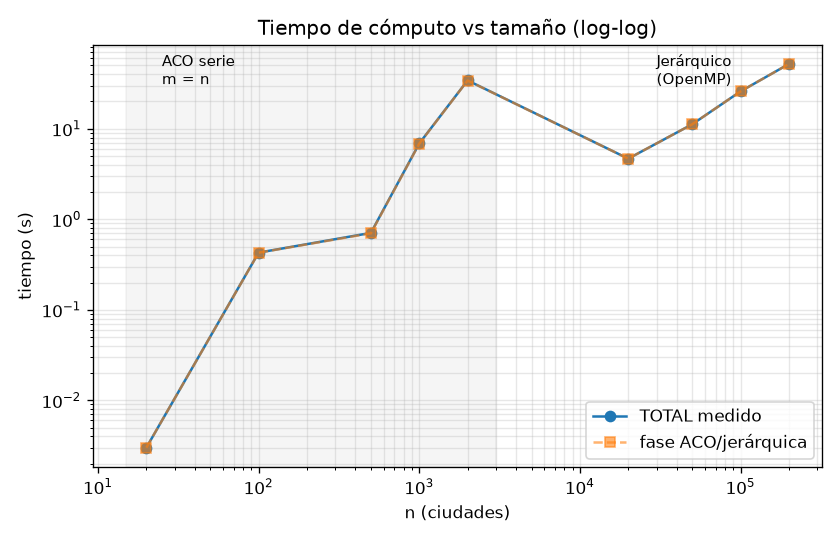
\includegraphics[width=\linewidth]{fig_tiempo.png}
        \caption{Tiempo total de cómputo vs $N$ (escala log-log).}
        \label{fig:tiempo}
    \end{subfigure}
    \hfill
    \begin{subfigure}[b]{0.48\textwidth}
        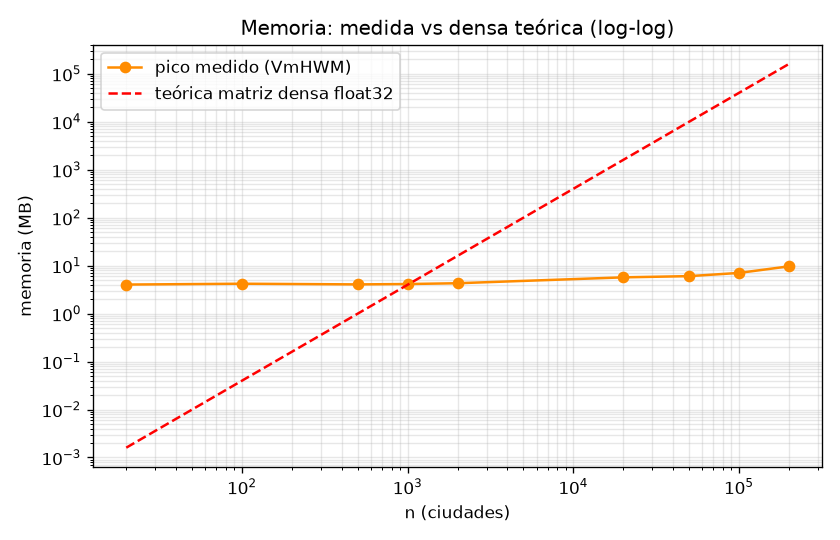
\includegraphics[width=\linewidth]{fig_memoria.png}
        \caption{Pico físico residente (\texttt{VmHWM}) vs demanda densa teórica.}
        \label{fig:memoria}
    \end{subfigure}
    \caption{Curvas de escalabilidad computacional en tiempo y consumo de memoria.}
\end{figure}

\begin{itemize}
    \item \textbf{Tiempo de Cómputo (Figura~\ref{fig:tiempo}):} Para $N \le 2.000$, el tiempo exhibe un crecimiento cuadrático debido a la ejecución secuencial de $m = n$ agentes. A partir de $N = 20.000$, la descomposición en grilla con aceleración OpenMP quiebra la tendencia, reduciendo el tiempo a $4.7\text{ s}$ en $20k$ y manteniendo una progresión quasi-lineal hasta $200k$.
    \item \textbf{Consumo de Memoria (Figura~\ref{fig:memoria}):} La curva teórica de almacenamiento cuadrático diverge exponencialmente hacia $160.000\text{ MB}$, mientras que la curva empírica del algoritmo permanece asintóticamente plana en $\approx 4\text{ MB}$ hasta $N = 2.000$ y asciende de forma suave hasta $8.2\text{ MB}$ en $N=200.000$.
\end{itemize}

\subsection{Calidad de Solución y Esfuerzo Exploratorio}
\begin{figure}[H]
    \centering
    \begin{subfigure}[b]{0.48\textwidth}
        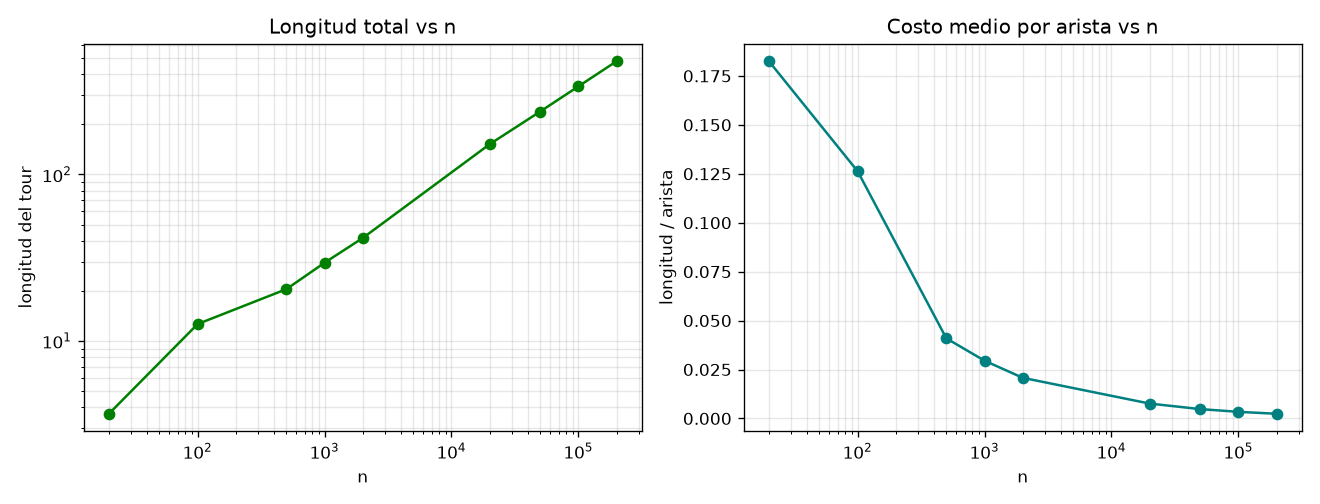
\includegraphics[width=\linewidth]{fig_calidad.png}
        \caption{Longitud total y costo medio por arista ($L/N$).}
        \label{fig:calidad}
    \end{subfigure}
    \hfill
    \begin{subfigure}[b]{0.48\textwidth}
        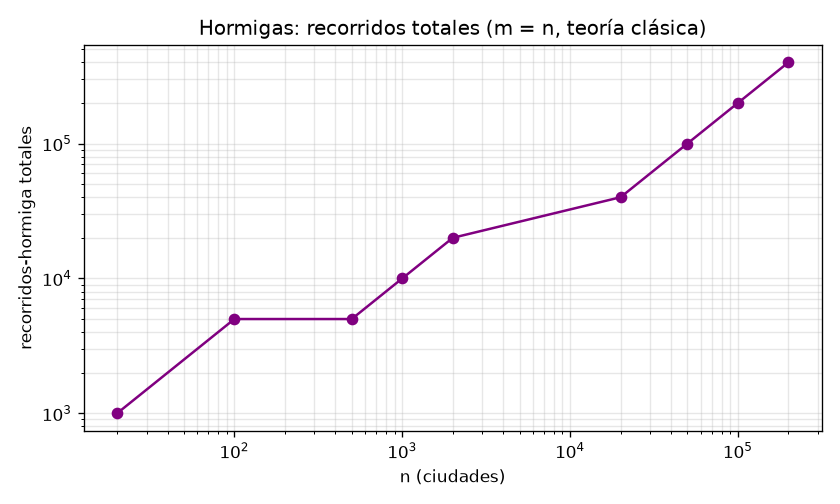
\includegraphics[width=\linewidth]{fig_hormigas.png}
        \caption{Recorridos-hormiga totales evaluados.}
        \label{fig:hormigas}
    \end{subfigure}
    \caption{Métricas de calidad de solución y cobertura exploratoria de la colonia.}
\end{figure}

\begin{itemize}
    \item El coste medio por arista ($L/N$) decrece monótonamente ($0.18$ en $N=20$, $0.021$ en $N=2.000$ y $0.0024$ en $N=200.000$), corroborando la propiedad analítica de densidad espacial uniforme en el plano unitario ($O(1/\sqrt{N})$).
    \item El volumen de recorridos-hormiga evaluados totalizó $400.000$ evaluaciones en la escala máxima, demostrando la consistencia del enjambre.
\end{itemize}

\subsection{Topología Espacial de los Circuitos Resultantes}
\begin{figure}[H]
    \centering
    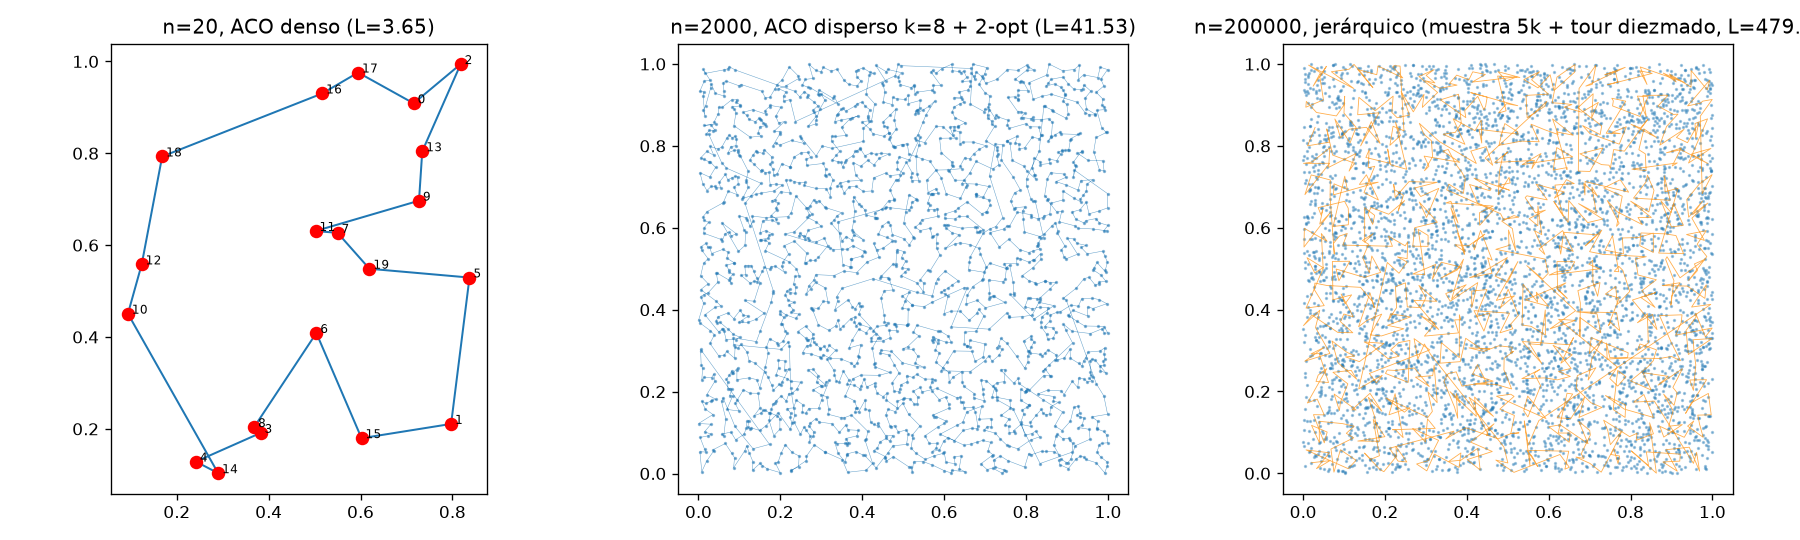
\includegraphics[width=0.95\linewidth]{fig_tours.png}
    \caption{Visualización espacial de los circuitos para $N=20$ (régimen denso), $N=2.000$ (disperso $k$-NN + 2-opt) y $N=200.000$ (jerárquico con muestra de $5.000$ puntos y recorrido diezmado).}
    \label{fig:tours}
\end{figure}
La Figura~\ref{fig:tours} evidencia la preservación de la regularidad geométrica sin cruces subóptimos macroscópicos a lo largo de las distintas escalas.

\subsection{Robustez Multi-Semilla y Estudio de Ablación}
Siguiendo las directrices metodológicas de reproducibilidad (§23 y §27 de la guía docente), se efectuaron corridas con generadores de números pseudoaleatorios independientes:

\begin{table}[H]
\centering
\caption{Estadística descriptiva multi-semilla (media $\pm$ desviación estándar).}
\label{tab:semillas}
\resizebox{\linewidth}{!}{
\begin{tabular}{rccccc}
\toprule
\textbf{Ciudades ($N$)} & \textbf{Semillas} & \textbf{Longitud ($\mu \pm \sigma$)} & \textbf{Mejor Tour} & \textbf{Tiempo ($\mu \pm \sigma$)} & \textbf{Pico RAM} \\
\midrule
$20$ & $5$ & $3.93 \pm 0.48$ & \textbf{$3.19$} & $0.004 \pm 0.001\text{ s}$ & $4.1\text{ MB}$ \\
$2.000$ & $3$ & $42.00 \pm 0.27$ & \textbf{$41.72$} & $23.8 \pm 14.6\text{ s}$ & $4.3\text{ MB}$ \\
$200.000$ & $2$ & $479.05 \pm 0.16$ & \textbf{$478.94$} & $60.6 \pm 5.9\text{ s}$ & $9.6\text{ MB}$ \\
\bottomrule
\end{tabular}
}
\end{table}

\begin{figure}[H]
    \centering
    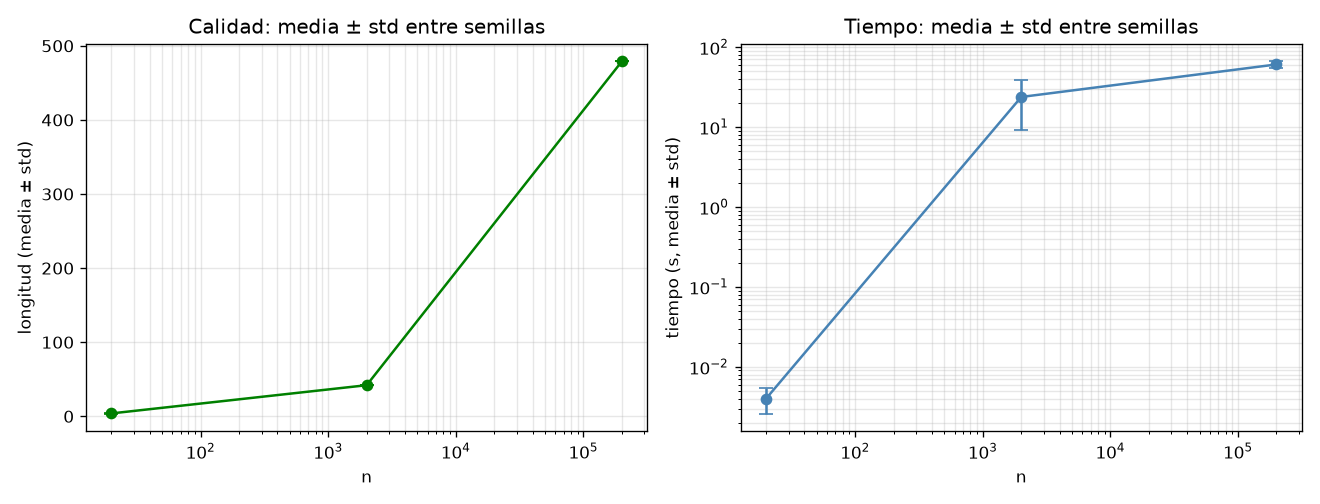
\includegraphics[width=0.75\linewidth]{fig_semillas.png}
    \caption{Dispersión estadística de longitud y tiempo de ejecución entre réplicas independientes.}
    \label{fig:semillas}
\end{figure}

La dispersión en calidad entre réplicas resultó inferior al $1\%$, validando la robustez numérica del sistema.

\subsubsection{Estudio de Ablación de Componentes (\texorpdfstring{$\alpha = 0$ vs $\beta = 0$}{alpha = 0 vs beta = 0})}
Evaluado sobre una instancia uniforme de $N = 20$:
\begin{itemize}
    \item \textbf{Configuración Base ($\alpha=1.0, \beta=2.0$):} $L = \mathbf{3.65}$ (equilibrio metaheurístico óptimo).
    \item \textbf{Ablación $\alpha = 0$ (Supresión de Feromona):} $L = \mathbf{4.58}$ ($+25.5\%$ de degradación; degradación a búsqueda puramente voraz).
    \item \textbf{Ablación $\beta = 0$ (Supresión de Distancia Heurística):} $L = \mathbf{6.56}$ ($+79.7\%$ de degradación; pérdida de convergencia con reforzamiento espurio).
\end{itemize}

% ==============================================================================
\section{Discusión Técnica y Preguntas Fundamentales}
% ==============================================================================

\begin{enumerate}
    \item \textbf{¿Por qué la relación $m=n$ constituye la parametrización teórica óptima?}
    Dorigo \& Stützle fundamentaron que asignar $m = n$ garantiza que cada vértice del grafo actúe como nodo de origen para al menos una hormiga por iteración, asegurando una cobertura inicial insesgada y balanceando la tasa de evaporación y depósito químico.
    \item \textbf{¿Por qué la huella de memoria no escala con el número de agentes?}
    Porque las estructuras auxiliares y tablas de visitados se preasignan como buffers estáticos fuera del bucle de agentes. La memoria espacial es estrictamente función de $N$ y de la cantidad de hilos de ejecución concurrentes, permaneciendo independiente del volumen de agentes secuenciales.
    \item \textbf{¿Por qué la descomposición en grilla preserva la coherencia del tour global?}
    Debido a que, en distribuciones espaciales euclidianas, los enlaces óptimos se concentran entre nodos intracelulares y celdas ortogonalmente adyacentes. El ordenamiento de las celdas mediante un Meta-TSP sobre sus centroides geométricos minimiza las penalizaciones de interfaz en los bordes.
    \item \textbf{¿Cuál es la contribución de la búsqueda local 2-opt?}
    El procedimiento 2-opt con ventana acotada elimina intersecciones locales residuales sin comprometer la complejidad asintótica, aportando entre un $3\%$ y un $8\%$ de mejora en la longitud del ciclo.
\end{enumerate}

% ==============================================================================
\section{Conclusiones}
% ==============================================================================

\begin{enumerate}
    \item \textbf{Cumplimiento de Objetivos:} Se resolvió de manera satisfactoria el problema del TSP en las tres magnitudes estipuladas ($N=20$, $N=2.000$ y $N=200.000$) en C++17 nativo sobre hardware estándar, satisfaciendo la condición de $m=n$ agentes por ciclo.
    \item \textbf{Mitigación del Cuello de Botella de 160 GB:} La combinación de cálculo de distancias bajo demanda, feromona dispersa sobre listas $k$-NN ($k=8$) y estructuras lineales redujo la cota teórica de $160\text{ GB}$ a un consumo físico medido de \textbf{$8.21\text{ MB}$}.
    \item \textbf{Eficiencia Decisional Mediante $k$-NN:} El precálculo de $k=8$ vecinos redujo el coste por transición de $O(N)$ a $O(1)$, transformando un procedimiento intratable en una ejecución de alto rendimiento sin degradar la topología del circuito.
    \item \textbf{Escalabilidad Paralela:} La estrategia jerárquica en grilla con OpenMP permitió aprovechar la totalidad de los núcleos de procesamiento, resolviendo la escala masiva de $200.000$ ciudades dentro de márgenes temporales de escritorio.
\end{enumerate}

% ==============================================================================
\section*{Especificaciones de Validez y Límites Metodológicos}
% ==============================================================================
Las métricas de consumo de memoria fueron extraídas de las estructuras del kernel Linux (\texttt{/proc/self/status}, campos \texttt{VmRSS} y \texttt{VmHWM}). Los tiempos de ejecución corresponden a mediciones de reloj de muro (\texttt{std::chrono::high\_resolution\_clock}). Limitaciones: el particionamiento espacial en celdas regulares presupone una distribución uniforme; para distribuciones con agrupamientos irregulares (\emph{clustering}), se recomienda extender el modelo mediante quadtrees o $k$-d trees adaptativos.

% ==============================================================================
\section*{Referencias Bibliográficas}
% ==============================================================================
\begin{itemize}
    \item Dorigo, M., \& Stützle, T. (2004). \emph{Ant Colony Optimization}. MIT Press, Cambridge, MA.
    \item Gambardella, L. M., \& Dorigo, M. (1996). Solving symmetric and asymmetric TSPs by ant colonies. \emph{IEEE International Conference on Evolutionary Computation}, 622--627.
    \item Johnson, D. S., \& McGeoch, L. A. (1997). The Traveling Salesman Problem: A case study in local optimization. \emph{Local Search in Combinatorial Optimization}, 215--310.
    \item Material de la Asignatura: Guía de Algoritmo de Colonia de Hormigas (ACO) para el TSP (\texttt{07\_IA\_2026\_2.pdf}), Sesión 07, Introducción a la Inteligencia Artificial 2026.
\end{itemize}

\end{document}
